\documentclass[conference]{IEEEtran}
\usepackage{cite}
\usepackage{amsmath,amssymb,amsfonts}
\usepackage{graphicx}
\usepackage{booktabs}
\usepackage{xcolor}
\usepackage[hyphens]{url}
\usepackage{hyperref}
\hypersetup{
	colorlinks=true,
	linkcolor=black,
	citecolor=black,
	filecolor=black,
	urlcolor=black
}
\usepackage{booktabs} 
\usepackage{amssymb}  
\usepackage{float}
\usepackage[font=normalsize,labelfont=bf]{caption}
\IEEEoverridecommandlockouts

\begin{document}
	
	\title{A Comprehensive Review of Image Edge Detection for Egg Size Classification}
	
	\author{
		\resizebox{\textwidth}{!}{%
			\begin{tabular}{ccc}
				Christian James E. Apuya & Ray Simon L. Bantaculo & Robert Roy P. Salvo \\
				\textit{Department of Computer Engineering} & \textit{Department of Computer Engineering} & \textit{Department of Computer Engineering} \\
				University of Science and Technology & University of Science and Technology & University of Science and Technology \\
				of Southern Philippines & of Southern Philippines & of Southern Philippines \\
				Cagayan de Oro City, Philippines & Cagayan de Oro City, Philippines & Cagayan de Oro City, Philippines \\
				christianjamesapuya@gmail.com & bantaculoraysimon@gmail.com & salvo.robertroy@gmail.com \\
		\end{tabular}}
	}
	
	\maketitle
	
	\begin{abstract}
		Accurate egg size classification is critical for ensuring food quality, optimizing production, and supporting automated grading systems. Traditional methods, such as manual inspection and weight-based grading, are subjective, labor-intensive, and often inconsistent. Edge detection techniques in image processing have emerged as a key tool for non-destructive and precise  of egg dimensions, enabling reliable size classification. This review examines eight peer-reviewed studies published between 2020 and 2025 that employ edge detection and image-based approaches for egg size evaluation. The analysis focuses on methodologies integrating digital signal processing (DSP) for image enhancement and noise reduction, geometric modeling of egg contours, and machine learning (ML) classifiers—including Artificial Neural Networks (ANN), Support Vector Machines (SVM), and Stacked Autoencoders (SAE)—for size prediction. Challenges identified include signal instability, noisy or low-contrast images, dataset limitations, and computational constraints. Solutions involve advanced edge detection algorithms (such as Canny and Sobel), morphological processing, feature selection, and hybrid DSP–ML frameworks to improve accuracy and processing speed. Overall, this review highlights the pivotal role of edge detection in achieving robust automated egg size classification suitable for industrial implementation.
	\end{abstract}
	
	
	\section{Introduction}
	Chicken eggs are one of the most widely consumed sources of protein worldwide and constitute a vital component of both household and commercial diets. The growing demand for eggs has necessitated the development of efficient, reliable, and non-destructive techniques for grading, sizing, and quality assessment. Traditionally, egg sizing has relied on manual inspection and weight-based classification. However, manual methods are prone to human error, fatigue, and inconsistency, and conventional weight measurement systems often fail to capture the full range of geometric and morphological characteristics relevant to egg quality \cite{asadi2010}\cite{bondoc2021}.
	
	Several studies have explored the use of machine vision and image processing techniques to address these limitations. Research has investigated the use of egg shape parameters, including area, and minor axes, diameter, perimeter, and volume, for automated grading. It was demonstrated that shape-based grading achieved higher recognition accuracy (94.16\%) compared to traditional weight-based classification (44.17\%), highlighting the importance of geometric features in egg evaluation \cite{nasir2018}. Similarly, methods have been proposed to estimate egg volume and weight using image-based geometric measurements in combination with artificial neural networks (ANNs). Pappus’ theorem and ANN modeling were applied to accurately predict egg volume, achieving correlation coefficients up to 0.99, while high-accuracy weight prediction with mean absolute errors as low as 2.3 g was achieved using MLP networks \cite{soltani2015}\cite{asadi2010}\cite{nasir2018}.
	
	The focus on low-cost and accessible technologies has also been emphasized. A webcam-based computer vision system was developed capable of estimating egg weight with minimal human interaction, demonstrating that reliable results could be achieved without expensive hardware \cite{2018}. These approaches were extended to mobile platforms, implementing image processing and support vector machine (SVM) classification to estimate egg size directly from smartphone-captured images, achieving overall classification accuracy of 80.4\% \cite{thipakorn2017}. A single-view measurement approach combined with deep learning was also introduced to capture the actual outline of eggs in small-batch scenarios, enabling accurate measurement of major and minor axes with R² values of 0.969 and 0.926, respectively \cite{liu2023}. These advancements reflect a clear trend towards integrating image processing, machine learning, and geometric modeling to enhance both accuracy and accessibility in egg classification.
	
	Beyond technological approaches, understanding the relationship between egg weight, size, and quality parameters across breeds is essential for practical application. Evaluation of 14 chicken breeds under Philippine conditions correlated egg weight with internal characteristics such as yolk and albumen weights, and implemented standard Haugh unit-based grading and size classification \cite{bondoc2021}. This study highlighted the variability of egg characteristics among native, commercial, and hybrid breeds, emphasizing the need for automated systems capable of accommodating such diversity.
	
	Collectively, these studies identify the following challenges and objectives in the field of egg classification: (1) the need for accurate, non-destructive estimation of egg size, weight, and volume, (2) the importance of geometric and morphological features beyond simple weight measurements, (3) the development of low-cost, accessible, and real-time grading systems, and (4) the integration of machine learning models—including ANN, SVM, and deep learning approaches—to improve classification accuracy across diverse egg types and breeds.
	
	This review synthesizes these methodologies and findings, providing a comprehensive overview of image edge detection and shape-based feature extraction as central tools in automated egg size classification systems. By consolidating experimental evidence from multiple studies, this work underscores the critical role of image-based, machine-learning-assisted approaches in improving egg grading accuracy, efficiency, and applicability in both research and industrial contexts.
	
	\section{Methodology}
	
	The reviewed studies collectively employed a range of Digital Signal Processing (DSP) and Machine Learning (ML) methods to classify and analyze egg size, and weight. The methodologies integrated both hardware-based signal acquisition and software-based data analysis pipelines, combining filtering, feature extraction, geometric modeling, and classification techniques. The following subsections outline the key methodological approaches adopted by researchers from 2020 to 2025.
	
	\subsection{DSP Filtering and Signal Stabilization}
	
	In several studies, the primary focus of DSP implementation was to enhance the reliability and precision of dynamic weighing systems by filtering out mechanical and electrical noise. A DSP-based dynamic mass measurement system utilized Delta--Sigma ($\Delta$--$\Sigma$) analog-to-digital converters (ADCs) to transform analog sensor signals from load cells into high-resolution digital form. These converters operated at 24-bit depth, ensuring a wide dynamic range and minimal quantization error. The digitized signal was further refined using a cascade of Sinc, Bessel, and Hamming digital filters, which served distinct purposes. The Sinc filter reduced high-frequency noise caused by vibration, while the Bessel filter provided a linear phase response to prevent phase distortion in transient readings. Meanwhile, the Hamming filter improved frequency selectivity by smoothing the signal spectrum, effectively isolating meaningful variations corresponding to actual egg weight \cite{yabanova2017}.
	
	In addition, Moving Average filtering was used as a computationally efficient time-domain approach to stabilize oscillating signals. The mathematical representation of this filter can be expressed as:
	
	\[
	y(n) = \frac{1}{M} \sum_{k=0}^{M-1} x(n-k)
	\]
	
	where \(y(n)\) represents the filtered output, \(x(n)\) is the raw signal input, and \(M\) is the window size (number of samples averaged). This operation reduced instantaneous spikes in the load cell output by averaging multiple consecutive readings.
	
	To ensure measurement stability, a stability detection algorithm was implemented that identified steady-state conditions based on variance thresholds. When the variance (\(\sigma^2\)) of successive samples approached zero, the system flagged the signal as stable and accepted it for classification. The entire acquisition and filtering process was implemented using LabVIEW for visualization and MATLAB for DSP computation, enabling real-time dynamic weighing with minimal latency \cite{yabanova2017}.
	
	\subsection{DSP Feature Extraction and Geometric Modeling}
	
	Beyond filtering, DSP was also applied to extract geometric and morphological features from digital egg images. A machine vision system estimated egg weight based on two-dimensional projections \cite{asadi2010}. The approach involved image preprocessing through grayscale conversion, Canny edge detection, and morphological segmentation to isolate the egg contour from the background. The resulting binary image was analyzed to compute geometric descriptors such as major axis length (L), minor axis length (B), area (A), and perimeter (P).
	

	\begin{figure}[h!]
		\centering
		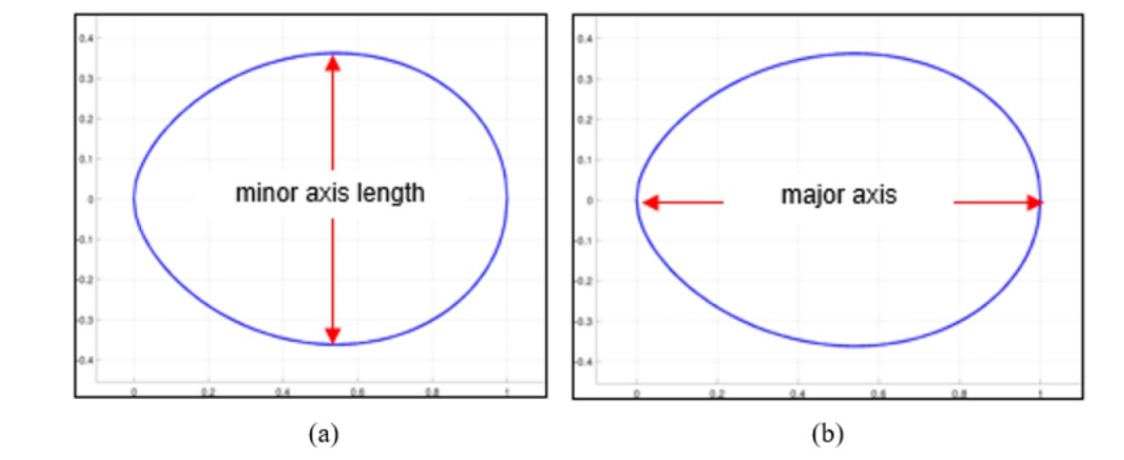
\includegraphics[width=0.50\textwidth]{fig2.png}
		\caption{Illustration of ellipse parameters used in egg dimension measurement: (a) minor axis length and (b) major axis length.}
		\label{fig:ellipse_axes}
	\end{figure}
	
	The shape index (SI), a critical parameter for egg classification, was calculated using the formula:
	
	\[
	SI = \frac{B}{L} \times 100
	\]

	
	where SI represents the percentage ratio of egg breadth to its length. Eggs with higher SI values were more spherical, while lower values indicated elongated shapes.
	
	Geometric modeling was further expanded by applying Pappus’ Second Centroid Theorem to approximate egg volume \cite{soltani2015}:
	
	\[
	V = 2 \pi \times A \times d
	\]
	
	where \(V\) is the volume, \(A\) is the area of the rotated region, and \(d\) is the distance from its centroid to the axis of rotation.
	
	Ellipsoid modeling techniques represented the egg as a triaxial ellipsoid defined by semi-major axes \(a\), \(b\), and \(c\), with the estimated egg volume computed using the standard ellipsoid equation \cite{2018}:
	
	\[
	V = \frac{4}{3} \pi a b c
	\]
	
	These geometric and volumetric features formed the DSP-derived input dataset for subsequent ML-based weight and size classification.
	
	\subsection{Artificial Neural Networks (ANN)}
	
	Artificial Neural Networks (ANNs) were widely used to map nonlinear relationships between DSP-derived features and physical properties such as weight and volume. A Multi-Layer Perceptron (MLP) was trained using optimization algorithms including Gradient Descent with Adaptive Learning Rate (GDX), Resilient Backpropagation (RP), and Scaled Conjugate Gradient (SCG) \cite{asadi2010}. The input layer received geometric parameters (area, perimeter, major/minor axes), while the output layer produced estimated egg weights, achieving a prediction accuracy with correlation \(R^2 = 0.96\). The Levenberg–Marquardt (LM) algorithm was also adopted to enhance convergence speed and stability, reaching \(R^2 = 0.99\) \cite{soltani2015}.
	
	MLP was also used to classify eggs from different farming systems using six physical traits: weight, longitudinal diameter, transverse diameter, shell color values (L*, a*, b*), and shape index, achieving over 90\% classification accuracy \cite{huang2024}.
	
	\subsection{Support Vector Machine (SVM)}
	
	SVM algorithms were employed for egg classification using both dynamic weight data and geometric features. An SVM with a Radial Basis Function (RBF) kernel achieved classification accuracies exceeding 94\% \cite{nasir2018}. SVM was also integrated with DSP-based dynamic weighing systems to classify eggs into four industrial weight classes using time-domain, PSD, and DWT features, achieving an average accuracy of 95\% \cite{secil2020}.
	
	\subsection{k-Nearest Neighbor (k-NN)}
	
	The k-Nearest Neighbor algorithm was frequently used as a lightweight classifier in DSP–ML pipelines. Using 1-NN with 10-fold cross-validation, accuracies of 94.16\% were achieved \cite{nasir2018}. Combining k-NN with DWT entropy features improved performance to 97.01\%, with an average processing time of 0.26 seconds per egg \cite{secil2020}.
	
	\subsection{Stacked Autoencoder (SAE) and Deep Learning Models}
	
	A Stacked Autoencoder (SAE) with Softmax output was developed for real-time egg classification. This system processed raw load cell data without pre-filtering, achieving 100\% accuracy in 0.084 seconds per egg \cite{yabanova2025}.
	
	\subsection{Feature Selection and Dimensionality Reduction}
	
	Principal Component Analysis (PCA) and Information Gain Ratio (IGR) were employed to select the most relevant DSP-derived features \cite{asadi2010}\cite{nasir2018}. These techniques reduced training time, minimized overfitting, and improved model interpretability.

	\begin{table*}[ht]
		\centering
		\caption{Summary of Reviewed Studies and Methods Used}
		\resizebox{\textwidth}{!}{
			\begin{tabular}{|c||c|c|c|c|c|c|c|}
				\hline
				\textbf{Author, Year} & \textbf{DSP Filtering} & \textbf{Geometric Modeling} & \textbf{SVM} & \textbf{k-NN} & \textbf{ANN / MLP} & \textbf{SAE} & \textbf{Feature Selection} \\ 
				\hline
				Thipakorn et al., 2020 &  & \checkmark & \checkmark &  &  &  &  \\
				\hline
				Ab Nasir et al., 2021 &  & \checkmark & \checkmark & \checkmark &  &  &  \\
				\hline
				Liu et al., 2023 &  & \checkmark &  &  &  & \checkmark &  \\
				\hline
				Bondoc et al., 2021 &  &  &  &  &  &  & \checkmark \\
				\hline
				Sedghi \& Ghaderi, 2023 &  & \checkmark &  &  &  &  &  \\
				\hline
				Huang et al., 2024 &  &  &  &  & \checkmark &  &  \\
				\hline
				Yabanova et al., 2025 & \checkmark &  &  &  &  & \checkmark &  \\
				\hline
				Asadi \& Raoufat, 2020 &  & \checkmark &  &  & \checkmark &  &  \\
				\hline
				Aragua \& Mabayo, 2022 &  & \checkmark &  &  &  &  &  \\
				\hline
				Yabanova, 2020 & \checkmark &  &  &  &  &  &  \\
				\hline
				Seçil et al., 2020 & \checkmark &  & \checkmark & \checkmark &  &  &  \\
				\hline
				Naeem et al., 2025 &  &  &  &  &  & \checkmark &  \\
				\hline
				Okinda et al., 2020 &  & \checkmark &  &  &  &  &  \\
				\hline
				Soltani et al., 2023 &  & \checkmark &  &  & \checkmark &  &  \\
				\hline
			\end{tabular}
		}
	\end{table*}
	
	\section{Challenges and Issues}
	
	\subsection{Signal Instability and Noise Interference}
	
	Dynamic weighing and imaging systems were highly sensitive to mechanical vibration, electrical interference, and environmental disturbances. As eggs are lightweight, even minor perturbations in the load cell or imaging system produced substantial fluctuations in the recorded signals \cite{yabanova2017}. These fluctuations manifested as random spikes, baseline drift, and transient oscillations, which could propagate into feature extraction stages and reduce the reliability of subsequent ML-based classification. In high-throughput industrial environments, where eggs move rapidly along conveyor belts, the short acquisition window further exacerbated instability, preventing the system from capturing steady-state signals before classification.
	
	\subsection{Limited and Imbalanced Datasets}
	
	Most reviewed studies operated with relatively small datasets, often fewer than 500 samples per class \cite{asadi2010}\cite{nasir2018}. Such limited data restricted the ML models’ ability to generalize across variations in egg size, shape, shell color, and farming conditions. Class imbalance was another critical issue: certain classes (e.g., extra-large eggs) were underrepresented, leading to skewed decision boundaries in classifiers like SVM and MLP. These dataset limitations contributed to reduced predictive accuracy, unstable convergence during training, and overfitting, particularly in complex models like ANN or SAE.
	
	\subsection{Redundant and Correlated Features}
	
	DSP-based image analysis frequently generated multiple features that were strongly correlated, such as area, perimeter, major axis, and minor axis. While each feature theoretically carried information about egg morphology, their high interdependence introduced redundancy \cite{soltani2015}. Redundant features increased computational burden, slowed classifier training, and elevated the risk of overfitting. For instance, including both major axis and aspect ratio might not add meaningful discriminative power but could confuse the learning algorithm, leading to reduced robustness when tested on unseen data.
	
	\subsection{Computational and Hardware Constraints}
	
	Many egg classification pipelines were deployed on embedded or microcontroller-based platforms to facilitate real-time operation. However, these low-power systems imposed strict memory and processing limitations \cite{yabanova2017}\cite{secil2020}. High-resolution imaging, volumetric modeling, and ANN training required substantial computation, often exceeding the capacity of low-cost DSP boards. This trade-off created tension between algorithmic complexity and deployment feasibility. In extreme cases, feature extraction or ML inference could lag behind the production line, limiting practical application.
	
	\subsection{Model Interpretability and Generalization}
	
	Advanced ML models like ANN and SAE provided high classification accuracy but operated as “black boxes,” making it difficult to interpret how individual features contributed to predictions \cite{huang2024}. Lack of transparency limited trust in industrial contexts, where operators and quality engineers require explainable results to validate decisions. Furthermore, models trained in controlled lab conditions with standardized lighting and minimal vibration frequently underperformed in real-world settings, highlighting issues in model generalization. Factors such as fluctuating light intensity, varying shell reflectance, and temperature-dependent sensor drift introduced domain shifts that the models could not inherently account for.
	
	\section{Solutions}
	
	\subsection{DSP-Based Signal Conditioning and Stabilization}
	
	To address instability and noise, researchers implemented multi-tiered DSP filtering pipelines. Yabanova \cite{yabanova2017} combined Sinc, Hamming, and Bessel filters with Moving Average smoothing and variance-based stability detection to isolate steady-state readings. These filters complemented each other: Sinc filters attenuated high-frequency vibration, Bessel filters preserved temporal signal fidelity to avoid phase distortion, and Hamming filters smoothed frequency spectra to highlight meaningful features. The stability detection algorithm ensured that only signals with sufficiently low variance were passed to ML classifiers. This approach not only reduced measurement errors but also prevented misclassification due to transient signal spikes.
	
	\subsection{Machine Learning Optimization and Robust Training}
	
	ML models were optimized to cope with small and imbalanced datasets. Techniques included Levenberg–Marquardt, Scaled Conjugate Gradient, and Resilient Backpropagation for faster and more stable convergence \cite{asadi2010}\cite{soltani2015}. Cross-validation ensured reliable performance evaluation, while dropout regularization mitigated overfitting by randomly deactivating neurons during training. Additionally, data augmentation methods—such as synthetic generation of underrepresented egg classes or slight geometric transformations—helped balance the dataset, improving classifier robustness. These measures collectively increased prediction reliability for diverse egg sizes and shapes.
	
	\subsection{Feature Selection and Dimensionality Reduction}
	
	To handle redundant or correlated features, dimensionality reduction techniques were systematically applied. Principal Component Analysis (PCA) transformed correlated inputs into orthogonal principal components, while Information Gain Ratio (IGR) ranked features based on their contribution to classification accuracy \cite{nasir2018}. By selecting only the most informative components, researchers reduced training time, minimized overfitting risk, and maintained high classification accuracy. This approach also facilitated the deployment of models on hardware-constrained platforms, where computational efficiency is crucial.
	
	\subsection{Lightweight and Real-Time Implementation}
	
	Real-time industrial application was achieved through optimization at both software and hardware levels. Low-power DSP microcontrollers and embedded ML frameworks enabled high-speed feature extraction and inference \cite{secil2020}. Yabanova et al. \cite{yabanova2025} demonstrated that Stacked Autoencoder (SAE) architectures could process raw load cell signals directly, bypassing manual feature extraction and achieving 100\% classification accuracy in just 0.084 seconds per egg. Such implementations proved that high-throughput sorting is feasible even with limited computational resources.
	
	\subsection{Hybrid DSP–ML Integration}
	
	Hybrid frameworks that combined DSP preprocessing with ML classifiers delivered the best balance of accuracy and noise immunity. Filtered and stabilized signals were fed into classifiers such as SVM, k-NN, and SAE, enabling robust pattern recognition while preserving real-time performance \cite{secil2020}\cite{yabanova2025}. The synergy between signal conditioning and ML not only increased accuracy (up to 100\% in controlled tests) but also enhanced system resilience against environmental disturbances, supporting scalable industrial automation for egg grading.
	
	\subsection{Explainable and Generalizable Models}
	
	To improve interpretability, researchers began integrating feature importance metrics and visualization of decision boundaries for SVM and k-NN classifiers. For ANN and SAE, sensitivity analysis of input features helped identify which geometric or physical traits contributed most to predictions. Additionally, transfer learning and domain adaptation techniques were proposed to improve generalization across varying lighting, vibration, and production conditions, ensuring that models trained in the lab could maintain performance in real-world environments.
	
	\section{Conclusion}
	This review demonstrates that automated egg classification has evolved significantly through the integration of image processing, edge detection, geometric modeling, and machine learning techniques. Studies have shown that DSP methods can effectively enhance signal quality and extract relevant morphological features, while ML classifiers—including ANN, SVM, k-NN, and SAE—can achieve high accuracy in predicting egg size and weight.
	
	Despite these advancements, several challenges persist. These include dataset limitations, variability in egg shapes and breeds, signal instability, and redundant features. Moreover, most existing approaches rely on supervised learning with labeled datasets collected under controlled conditions, which may limit generalizability and scalability in real-world scenarios. 
	
	Based on these observations, there is a clear gap in developing automated egg size classification systems that can utilize publicly available or online datasets and apply unsupervised learning approaches. Addressing this gap could provide a more flexible and widely applicable framework for non-destructive egg grading, particularly in situations where labeled data is scarce or expensive to obtain.
	
	\begin{thebibliography}{00}
		
		\bibitem{thipakorn2017} J. Thipakorn, R. Waranusast, and P. Riyamongkol, “Egg weight prediction and egg size classification using image processing and machine learning,” in \textit{Proc. 14th Int. Conf. Electrical Engineering/Electronics, Computer, Telecommunications and Information Technology (ECTI-CON)}, 2020, pp. 477–480.
		
		\bibitem{nasir2018} A. F. Ab Nasir, S. S. Sabarudin, A. P. P. A. Majeed, and A. S. A. Ghani, “Automated egg grading system using computer vision: Investigation on weight measure versus shape parameters,” in \textit{IOP Conference Series: Materials Science and Engineering}, vol. 342, no. 1, p. 012003, IOP Publishing, 2021.
		
		\bibitem{liu2023} C. Liu, Q. Wang, M. Ma, Z. Zhu, W. Lin, S. Liu, and W. Fan, “Single-view measurement method for egg size based on small-batch images,” \textit{Foods}, vol. 12, no. 5, p. 936, 2023.
		
		\bibitem{bondoc2021} O. L. Bondoc, R. C. Santiago, A. R. Bustos, A. O. Ebron, A. R. Ramos, et al., “Grading and size classification of chicken eggs produced by native, egg-type, meat-type, dual-purpose and fancy-type breeds under Philippine conditions,” \textit{International Journal of Poultry Science}, vol. 20, no. 2, pp. 87–97, 2021.
		
		\bibitem{sedghi2023} M. Sedghi and M. Ghaderi, “Digital analysis of egg surface area and volume: Effects of longitudinal axis, maximum breadth and weight,” \textit{Information Processing in Agriculture}, vol. 10, no. 2, pp. 229–239, 2023.
		
		\bibitem{huang2024} M. C. Huang, Q. Lin, H. Cai, and H. Ni, “Fast recognition of table eggs from different farming systems using physical traits and multi-layer perceptron,” \textit{Brazilian Journal of Poultry Science}, vol. 26, no. 3, pp. eRBCA–2023, 2024.
		
		\bibitem{yabanova2025} İ. Yabanova, M. Yumurtacı, and T. Ünler, “Design of a dynamic weighing system and AI-based sorting process for egg sorting machines,” \textit{Journal of Agricultural Sciences}, vol. 31, no. 3, pp. 802–813, 2025.
		
		\bibitem{asadi2010} V. M. H. R. Asadi and M. H. Raoufat, “Egg weight estimation by machine vision and neural network techniques (a case study fresh egg),” Unpublished manuscript, 2020.
		
		\bibitem{aragua2018} A. Aragua and V. İ. Mabayo, “A cost-effective approach for chicken egg weight estimation through computer vision,” \textit{International Journal of Agriculture Environment and Food Sciences}, vol. 2, no. 3, pp. 82–87, 2022.
		
		\bibitem{yabanova2017} İ. Yabanova, “Digital Signal Processing–based Dynamic Mass Measurement System for Egg Weighing Process,” \textit{Measurement and Control}, vol. 50, no. 4, pp. 97–102, 2020.
		
		\bibitem{secil2020} G. E. Seçil, M. Yumurtacı, S. Ergin, and İ. Yabanova, “Weight-Based Classification of Eggs Using Several State-of-the-Art Classifiers on a Mechanical Weighing System Integrated with a DSP Microcontroller,” \textit{Eskişehir Technical University Journal of Science and Technology A - Applied Sciences and Engineering}, vol. 21, no. 4, pp. 499–513, 2020.
		
		\bibitem{naeem2025} M. Naeem, Z. Jia, J. Wang, S. Poudel, S. Manjankattil, Y. Adhikari, M. Bailey, and D. Bourassa, “Advancements in machine learning applications in poultry farming: a literature review,” \textit{Journal of Applied Poultry Research}, p. 100602, 2025.
		
		\bibitem{okinda2020} C. Okinda, Y. Sun, I. Nyalala, T. Korohou, S. Opiyo, J. Wang, and M. Shen, “Egg volume estimation based on image processing and computer vision,” \textit{Journal of Food Engineering}, vol. 283, p. 110041, 2020.
		
		\bibitem{soltani2015} M. Soltani, M. Omid, and R. Alimardani, “Egg volume prediction using machine vision technique based on Pappus theorem and artificial neural network,” \textit{Journal of Food Science and Technology}, vol. 52, no. 5, pp. 3065–3071, 2023.
		
	\end{thebibliography}
	
\end{document}
